\documentclass[border=0.8ex,svgnames,tikz]{standalone}
\usepackage{amsmath,mathtools}
\usepackage{fontspec}
\setmainfont{Source Serif 4}
\setsansfont{Source Sans 3}
\setmonofont{Source Code Pro}
\usetikzlibrary{calc,positioning}
\begin{document}
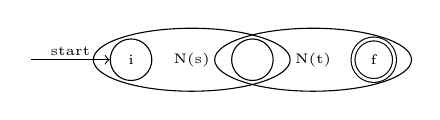
\begin{tikzpicture}
  \node[text width=-3em](Start){};
  \node[circle, draw=black, minimum width=15pt, minimum height=15pt, right=of Start](RI){\tiny i};
  \node[circle, draw=black, minimum width=15pt, minimum height=15pt, right=of RI](MID){\tiny \quad};
  \node[circle, double, double distance=1pt, draw=black, minimum width=15pt, minimum height=15pt, right=of MID](RF){\tiny f};

  \path[->]
  (Start) edge node[above=-2pt]{\tiny start} (RI)
  (RI) edge[draw=none] node{\tiny N(s)} (MID)
  (MID) edge[draw=none] node{\tiny N(t)} (RF);

  \draw ($(RI)!0.5!(MID)$) ellipse (1.25 and 0.4);
  \draw ($(MID)!0.5!(RF)$) ellipse (1.25 and 0.4);
\end{tikzpicture}
\end{document}
